
%(BEGIN_QUESTION)
% Copyright 2011, Tony R. Kuphaldt, released under the Creative Commons Attribution License (v 1.0)
% This means you may do almost anything with this work of mine, so long as you give me proper credit

Tegn inn de nødvendige koblingene for å koble to nærhetsbrytere og to solid-state releer til en Allen-Bradley MicroLogix 1000 PLC (model 1761-L10BWA, med 6 DI-er som kan være sourcing eller sinking og 4 DO med potensialfrie relekontakter. Koble nærhetsbryteren som er sourcing (PNP) til inngang \texttt{I:I/0}, bryteren som er sinking til \texttt{I:I/4}, og de to solid state-releene til \texttt{O:O/1} og \texttt{O:O/2}:


$$\includegraphics[width=15.5cm]{i04524x01.eps}$$

\vskip 20pt \vbox{\hrule \hbox{\strut \vrule{} {\bf Suggestions for Socratic discussion} \vrule} \hrule}

\begin{itemize}
\item{} What advantages do {\it solid-state} relays enjoy over their electromechanical counterparts?
\item{} Can these solid-state relays switch DC, AC, or both?
\item{} Identify how the behavior of a TRIAC differs from that of a bipolar or field-effect transistor.
\end{itemize}

\underbar{file i04524}
%(END_QUESTION)





%(BEGIN_ANSWER)

Note: standard electronic proximity switch wiring color codes are as follows:

\begin{itemize}
\item{} {\bf Brown} = Positive (+) DC supply
\item{} {\bf Blue} = Negative ($-$) DC supply
\item{} {\bf Black} = Signal output
\end{itemize}

This is just one possible solution:

$$\includegraphics[width=15.5cm]{i04524x02.eps}$$
%$$\includegraphics[width=15.5cm]{i04524x03.eps}$$
Note that this solution shows the two solid-state relays connected to the PLC output such that the PLC {\it sinks} current from the relays.  Since no instructions were given on wiring the PLC outputs, this is just one possible solution out of many.

%INDEX% PLC, I/O: discrete I/O device wiring
%INDEX% Switch, proximity: sourcing versus sinking output
%(END_ANSWER)





%(BEGIN_NOTES)


%(END_NOTES)


